\documentclass[a4paper]{article}
\usepackage{graphicx} 
\usepackage{hyperref}
\usepackage{booktabs}
\usepackage{listings}
\usepackage{geometry}
\usepackage{booktabs}
\usepackage{multirow}

\lstset{
  basicstyle=\ttfamily,
  columns=fullflexible,
  frame=single,
  breaklines=true,
  postbreak=\mbox{{$\hookrightarrow$}\space},
}

\title{Mining Experimental Data in Materials Research with Large Language Models}
\author{Luca Foppiano}
% Potential Co-authors: Pedro Ortiz, Guillaume Lambard, Ishii, Amagasa, Lopez
\date{June 2023}

\begin{document}

\maketitle

\section{Introduction}

Mining experimental data from papers has become increasingly popular in materials science due to the vast amount of information available and the need for accelerating materials discovery using data-driven techniques.

% Why is important?
A substantial volume of experimental data needs to be gathered, primarily sourced from findings published in scientific articles.
Nonetheless, this data comes in various forms: unstructured textual content and structured tables and graphs, adding complexity to the extraction process. 
As a result, many projects still depend on manual data extraction.
While there are a few extensive structured databases containing accumulated experimental data, they remain limited in number when compared to the numerous projects within the field of materials science research.

% Why is challenging?
In materials science, addressing issues related to data quality and interpretation demands meticulous curation and specialised domain knowledge.
When dealing with scientific texts originating from materials research articles, one must possess a profound comprehension of the laws of physics and the skill to navigate through a maze of jargon, intricate vocabularies, and specialised terminology unique to each sub-domain. 
For instance, in the field of superconductors, experts in the domain categorise materials into classes, which are sometimes defined arbitrarily, blending compound-based classes like \textit{cuprates} and \textit{iron-based} materials with phenomenon-based classes like \textit{fermions}. 
Moreover, there exists substantial confusion due to the frequent overuse of certain terms. For instance, the acronym "TC" is often employed to denote "Temperature Curie," while "Tc" signifies "superconducting critical temperature". 
These sub-domain-specific conventions pose a significant challenge when attempting to create structured datasets that can function effectively across various sub-domains.

% What is the problem we are trying to solve? 
The advent of Large Language Models (LLM) has ushered in a new era of technology with immense potential, ranging from the capacity to link concepts to engaging in conversational reasoning.
LLM models offer a more efficient approach based on a centralised API offering performance superior to most of the off-the-shelf solutions. 
As a consequence, previous limitations such as the context window to a maximum of 512 tokens of small scale model (SSM) such as BERT. 
At the time of writing this article, "chatgpt-3.5-turbo" allows a context window of 4096 tokens, "gpt4-turbo" reaching up to 128k tokens. Anthropic Claude 2.1, recently released claims a context window above 200k tokens.  
Such models are capable of digesting entire articles, and even larger reports, although is not clear how effective the LLM is to retain information from any part of the document.
The demand for structured data necessitates the extraction of more intricate information in a flexible manner. 
LLMs present a valuable opportunity to expedite the development of Text and Data Mining (TDM) processes that can be described as processing free text. 
Although achieving this objective is still a considerable challenge, this study aims to assess LLMs' ability to comprehend, manipulate, and reason with complex information that demands substantial background knowledge as in Materials Science. 

% Goals 
The objectives of this work can be summarised in the following questions: 
\begin{itemize}
    \item \textit{How effectively can LLMs extract materials science-related information?}
    \item \textit{To what extent can LLMs engage in reasoning to relate complex concepts?}
    % \item \textit{What volume of information is necessary to use, to bridge the gap between LLMs and specialized SLMs models?}
\end{itemize}

% Method
We observe that the fundamental components of materials science knowledge can be grouped into two main classes: materials and properties expressions. 
Properties (e.g. critical temperature, 4K) are expressed using quantities and measurements: they exhibit a structured format, including modifiers, values, and units, with a wide range of potential values. 
In contrast, materials are conceptually fluid and often depend on the specific domain. They may necessitate a substantial amount of accompanying text for a comprehensive description, which can encompass details like doping ratio, substrate, and other characteristics. 
From a chemical standpoint, materials are defined by their chemical formula. 
However, in practice, scientists frequently employ names such as commercial names, well-known terms, or invented designations to describe samples, all of which serve to streamline information in research papers. Nonetheless, conveying such definitions unambiguously can be challenging.


% NER
To answer the first research question, \textit{ow effectively can LLMs extract materials science-related information} we compare a selection of LLMs on tasks of Named Entities Recognition (NER) of both materials and properties.  
We define the baseline as the Small Language Models (SLMs) based on BERT-flavoured encoder~\cite{beltagy2020scibert}. 
The interaction with the LLMs is then performed using three different strategies: zero-shot, few-shot, and fine-tuning (instruct-based generation). 
% For the specific case of few-shot generation, the way information is provided can be implemented with three strategies: a) provide a definition in the prompt, b) provide examples in the prompt, and, c) provide both. 
% It is crucial to emphasise the significant data requirements for both few-shot and instruct-based generation, for achieving satisfactory results in tasks that involve handling complex vocabulary, particularly in the context of materials science.

% RE
Answering the second question, \textit{To what extent can LLMs engage in reasoning to relate complex concepts?} requires us to evaluate the ability to extract relations given a list of entities that are already pre-defined. 
The baseline is defined by a rule-based approach we have developed in previous work~\cite{lfoppiano2023automatic} and based on the same dataset. 
The interaction with the LLMs is performed only using: zero-shot, few-shot and fine-tuning.  
 
% Evaluation matching 
While classical SMLs classify each token in the input, the comparison with the expected dataset is a matter of matching between two values. Soft-matching can be used to ignore small differences. 
With generative models, the output tokens might be constructed with constructs that are completely different from the original input sequence. 
In general cases, is possible to compare using semantic models that compare the vectorised equivalent of the two sequences~\cite{reimers2019sentencebert}. 
However, concepts such as the material's expressions require running the comparison using some normalised expression. 
We propose a novel approach for evaluating material names that normalise materials at their chemical formula before the pairwise comparison of each element. 

We summarise the contributions that are provided in this work as follows: 

\begin{itemize}
    \item We evaluated and compared LLM on extracting information such as Named Entities Recognition (NER) in both materials expressions and properties extraction, using zero-shot, few-shot and fine-tuned (or instruction-tuning) generation,
    \item We evaluated LLMs on Relation Extraction (RE) of information from different nature, such as materials, properties and conditions
    \item We propose a novel approach for evaluating IE tasks applied to materials entities which use formulas matching via pairwise element comparison.
\end{itemize}


\section{Related Work}

Numerous studies have delved into the evaluation of Large Language Models (LLMs) within the scientific domain. However, the rapid advancement in this field poses a significant challenge in synthesising all relevant background studies. Initial assessments of ChatGPT highlighted its proficiency in general tasks, though it fell short in specific areas compared to state-of-the-art (SOTA) models~\cite{kokon2023chatgpt}. In the biomedical domain, the early Curie model struggled to outperform BioBERT in few-shot generation scenarios~\cite{moradi2022gpt3}.

A study on correlation and causation detection~\cite{jin2023large} observed that ChatGPT's performance did not surpass that of a random model. Additionally, challenges emerged in named entity recognition and classification (NERC) for historical documents, attributed to potential issues with internet data reliance and inconsistent entity definitions across guidelines~\cite{gonzalez2023yes}.

In contrast to small language models (SLMs) like Roberta-large, a study by Ma et al.~\cite{ma2023large} found that LLMs, including ChatGPT, struggled with tasks such as NER, relation extraction (RE), and event detection (ED) in few-shot generation scenarios. However, they proposed a hybrid approach, combining both LLMs and SLMs, demonstrating improved performance on tasks requiring specific knowledge or extensive context.

Another investigation~\cite{tang2023struc} found that GPT3.5-turbo and GPT4 faced challenges in generating complex output structures like tables, achieving only 3-9\% accuracy on specific formatting constraints. Fine-tuning on a smaller model, LLaMA-7B, significantly improved performance on both seen and unseen structured text generation.
In materials,~\cite{hatakeyama2023prompt} explore GPT-4’s potential in chemical tasks and other reasoning related to chemical information.

Notably, the requirement for a valid JSON output, as reported in this study, introduces additional challenges not commonly addressed in related works focused on conversational aspects~\cite{lin2023llmeval, min2023factscore}.

\section{Method}
\label{sec:method}
We assessed three OpenAI LLM models—ChatGPT (gpt-3.5-turbo or gpt-3.5-turbo-0611), GPT-4 (gpt-4), and GPT-4-turbo (gpt-4-0611-preview)—chosen for their pioneering and advanced capabilities.

Our evaluation focused on NER and RE tasks, employing various generation approaches (few-shot, zero-shot, and fine-tuned). 
We compared results with respective baselines, utilising SuperMat~\cite{lfoppiano2021supermat} for NER of materials and MeasEval~\cite{harper2021semeval2021} for properties extraction. SuperMat relations were employed for evaluating RE between materials and properties.
Baseline scores were established using a SciBERT-based encoder and RE rule-based algorithm~\cite{lfoppiano2023automatic} for material-related extractions. Grobid-quantities~\cite{foppiano2019quantities} served as the baseline for NER on properties extraction, compared against MeasEval.
Results were formatted in valid JSON through the LangChain library. Evaluation scores, encompassing Precision, Recall, and F1-score, were derived from pairwise comparisons between predicted and expected entities. Precision gauges accuracy, recall assesses information capture, and F1-Score harmonizes precision and recall.

The presented evaluations condense F1 scores over three extraction runs; detailed values are available in the Supplementary Material section.

\subsection{Named Entities Recognition}
\label{sec:ner}
The NER task consists of identifying relevant entities: materials, expressed in a multitude of expressions~\cite{lfoppiano2021supermat}, or properties, expressed as physical quantities~\cite{foppiano2019quantities}. 

We implemented the pairwise comparison using four different matching approaches: 
\begin{itemize}
    \item \textbf{strict}: exact matching
    \item \textbf{soft} matching using Ratcliff/Obershelp with a threshold at 0.9
    \item \textbf{sbert} using Sentence BERT with cross-encoder~\cite{reimers2019sentencebert} to compare the contextual embeddings representation of the two sequences. This approach aims to capture the semantic differences and similarities between the two sequences. Threshold at 0.8.
    \item \textbf{formula matching} a novel method to compare materials expressions via formula normalisation and element-by-element exact matching.
\end{itemize}

The prompt is designed following the OpenAI template composed by a \textit{system prompt} and a \textit{user prompt} and we concatenated them for all other models not supporting such an approach.

The NER task for materials extraction using zero-shot was described using a prompt containing both definitions and examples of the materials as they are described in the annotation guidelines\footnote{Accessible at \url{https://supermat.readthedocs.io}} used to construct SuperMat~\cite{lfoppiano2021supermat}. 
Following is an example of a template for materials extraction: 

\begin{lstlisting}[caption=Generic system prompt common to all requests]
Use the following pieces of context to answer the user's question. 
If you don't know the answer, just say that you don't know, don't try to make up an answer. 
----------------
{text}
\end{lstlisting}


\begin{lstlisting}[caption=User prompt designed for extracting materials from text]
What are the superconductor materials mentioned in the text? 
Only provide the mention of the materials. Avoid repetition. 

The material can be expressed as follows:
- chemical formula with variables not substituted, like La(1-x)Fe(x),
- chemical formula with substitution variables like Zr 5 X 3 (X = Sb, Pb, Sn, Ge, Si and Al)
- with complete or partial abbreviations like (TMTSF) 2 PF 6,
- doping rates are represented as variables (x, y or other letters) appearing in the material names. These values can be used to complement the material variables (e.g. LaFexO1-x).
- doping rates as percentages, like 4% Hdoped sample or 14% Cu doped sample
- material chemical form with no variables e.g. LaFe03NaCl2 where the doping rates are included in the name
- chemical substitution or replacements, like (A is a random variable, can be any symbol): A = Ni, Cu, A = Ni, Ni substituted (which means A = Ni)
- chemical substitution with doping ratio, like (A is a random variable, can be any symbol): A = Ni and x = 0.2

If you don't know the answer, just say you don't know, don't try to make up an answer.
\end{lstlisting}

The same approach was followed for the NER on properties extraction by adding in the prompt template the description from the MeasEval guidelines\footnote{Accessible at \url{https://github.com/lfoppiano/MeasEval/tree/main/annotationGuidelines\#basic-annotation-set}}. Following is an example of a user prompt template. 

\begin{lstlisting}[caption=User prompt designed for extracting properties from text. ]
Quantity is either a Count, consisting of a value, or a Measurement, 
consisting of a value and usually a unit. A Quantity can additionally include optional Modifiers like tolerances.
Include relevant text that indicates the application of a modifier, such as "between" "less than" "approximately", 
or symbols such as ">" or "~" if they are contiguous with the span. Ignore them if they are separated by additional text.
 
Example: "The soda can's volume was 355 ml", the quantity is "355 ml".

Extract all the Quantities in the text.
\end{lstlisting}

We implemented the few-shot generation using the same prompts and injecting a list of hints or suggestions that are extracted from the text using the respectively specialised models based on the SciBERT encoder: grobid-superconductors~\cite{lfoppiano2023automatic}, and grobid-quantities~\cite{foppiano2019quantities}, respectively.
Since the suggestions are provided by another model, they are not correct 100\% of the time, we stressed in the prompt that they are examples or hints, that the LLMs could ignore. 
This is implemented by adding the following information at the end of the prompts, both for materials and measurements:

\begin{lstlisting}[caption=Few shot information suffixed to the prompt]
[...]
Here are some examples appearing in the text: {hints}
[...]
\end{lstlisting}


\subsubsection{Formula matching}

The matching of materials is tricky with generative models. Encoder and sequence labelling models classify tokens, the output remains unchanged from the input making it easier to evaluate and compare. 
Performing entity extraction with generative models might result in greatly different output, yet, semantically the same as the input. For this reason, other works~\cite{taylor2022galactica} used a manual approach for part of their evaluation. 
At the time of writing this article, we were not aware of any approach that is tailored for material expressions. 
The use of sentence BERT, which was trained on general text, does not guarantee that the embeddings of materials are calculated correctly and, therefore that the final match is meaningful. 
Researchers often use sets of variables to avoid explicitly writing down a list of formulas that are almost identical except for one element, for example. This is very common when the discussion is about replacing one rare earth element with others (e.g. \texttt{RE x La 1-x O 7 with RE = Y, Pr,Sm,Eu,Gd and x = 0.1, 0.2}). 
For this reason, we propose a new novel approach for evaluating extracted material names through element-by-element pairwise comparison on a normalised formula: \textit{formula\_matching}.

\begin{figure}[ht]
  \centering
  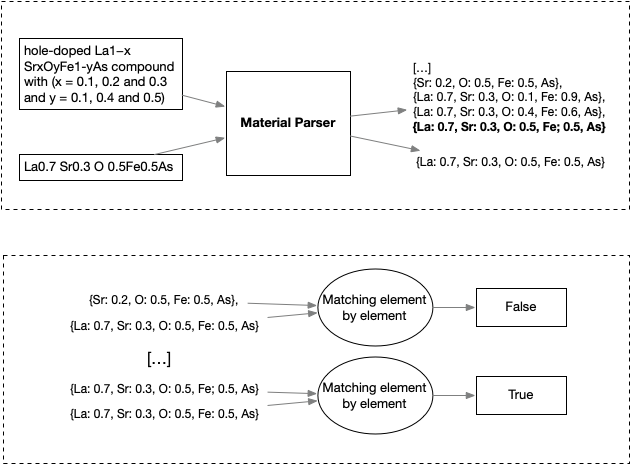
\includegraphics[width=1\textwidth]{figures/formula-matching-schema.png} 
  \caption{Two materials that appear to have a very different composition, are, in reality overlapping. (Top) Summary of the Material Parser. More information is available in~\cite{lfoppiano2023automatic}. (Bottom) The pairwise comparison of each chemical formula is performed element-by-element.  }
  \label{fig:formula-matching-schema}
\end{figure}

This method is an extension of the strict matching and is triggered only if the two input strings are not the same. 
In such case, as illustrated in Figure~\ref{fig:formula-matching-schema}, the material expressions to be compared are passed to a material parser we have developed in our previous work~\cite{lfoppiano2023automatic} which normalises them down to their formula (Figure~\ref{fig:formula-matching-schema} top). 
The material parser has been developed to digest a relatively high amount of noisy material expressions and try to figure out the best way to parse it. 
The expected output is a structure composed of several elements and the chemical formula is presented both as a raw string and as a dictionary composed of elements and the respective amount. 
Once these structures are obtained, we then compared element by element as illustrated in Figure~\ref{fig:formula-matching-schema} bottom.

\subsection{Relation Extraction}
\label{sec:re}
The baseline is established by a rule-based algorithm that we used in our previous work~\cite{lfoppiano2023automatic} which was evaluated with SuperMat and for which we report the aggregated result in Section~\ref{sec:re}. 

For evaluating the relation extraction task, we provide a list of entities and ask the LLM to group them based on their relation. 
Differently from the NER task, the LLM is expected to reuse information that is passed in the prompt to compose the response: non-matching information is considered incorrect. 
However, we also provide evaluation scores based on soft matching whose description is available in Section~\ref{sec:results}. 

We evaluated three types of generation: zero-shot generation, few-shot generation, and fine-tuned generation. 
The same considerations discussed before are valid for system and user prompts. 
The system prompt for the RE task is modified to provide a detailed description of the task beforehand. 

\begin{lstlisting}[caption=System prompt]
You are useful assistant, who knows about materials science, physics, chemistry and engineering.
You will be asked to compute relation extraction given a text and lists of entities. 
If you are not sure, don't try to make up your answer, just answer "None". 
\end{lstlisting}

The task description is further repeated in the user task with the addition of specific rules that act to avoid the return of incorrect JSON format. 
In particular, we want to avoid: relations from entities not supplied in the input (this could lead to any complex format), and relations blocks that are empty. 

\begin{lstlisting}[caption=Relation extraction using zero-shot generation]
Consider the following text in between triple quotes: 
"""
{text}
"""

Find the relations between lists of entities of different classes. 
Apply strictly the following rules:  
    - if the material is not specified, ignore the relation block,
    - if tc is not specified in absolute values, ignore the relation block 
    
Following are the lists of entities: 
{entities}
\end{lstlisting}

The few-shot prompt was just a modified zero-shot prompt that contained two static examples of input, and output. 

\begin{lstlisting}[caption=Few-shot generation for extracting relations from lists of entities]
Given a text between triple quotes and a list of entities, find the relations between entities of different classes: 
"""
{text}
"""

{entities}

--------
Example: 
The researchers of Mg have discovered that MgB2 is superconducting at 29 K at ambient pressure.

entities:
 materials: MgB2, Mg
 tcs: 29K
 pressure: ambient pressure
 
Result: 
 material: MgB2, 
 tc: 29K, 
 pressure: ambient pressure
 
--------
Apply strictly the following rules:  
    - if the material is not specified, ignore the relation block,
    - if tc is not specified in absolute values, ignore the relation block 
\end{lstlisting}

% The fine-tuned was implemented using the prompt used for the zero-shot generation provided to a model that was fine-tuned using a partition of SuperMat (344 examples for training and 148 examples for testing) and evaluated with the rest (88 examples). One example represents a unique paragraph with multiple relations within.

The entity list provided to the LLM may be extracted in order of appearance, therefore it could happen that a model that just generates relations in order, may obtain a high score that does not represent its actual relation inference capabilities. 
For this reason, for each model and generation type, we provide two versions: \emph{non-shuffled} where the entities are provided as they appear, and \emph{shuffled} where the entities are shuffled randomly before they are provided to the prompt. 

\subsection{Consideration about the fine-tuning}

We fine-tuned the gpt3.5-turbo model using the OpenAI platform which ingested a couple of files for training and testing (Table~\ref{tab:amount-data-fine-tuned}) and generated a new model in a few hours.
Since the MeasEval dataset is of medium size, we employed another dataset we developed in the past~\cite{foppiano2019quantities} for the fine-tuning of the NER for properties extraction. 

\begin{table}[htbp]
    \centering
    \label{tab:amount-data-fine-tuned}
    \caption{Amount of data used for training the fine-tuned models.}
    \begin{tabular}{lccc}
        Task & Dataset & \# Training & \# Test \\
        \toprule
        NER & SuperMat   & 1639 & 703 \\
        NER & Quantities & 485 & 208 \\
        RE  & SuperMat   & 344 & 148 \\
        \bottomrule
    \end{tabular}
\end{table}

The requirement to obtain a valid machine-readable JSON format resulted to be the main point of failure when using a fine-tuned model. 
In other words, the fine-tuned models were not able to provide valid JSON in output, we hypothesised that the cause could be the lack of training examples. 
We solved this issue by generating the fine-tuned training data using a pseudo format structured with spaces and break-lines that could be handled more simply by the model. 
Following is an example of the fine-tuning of a RE task: 
\begin{lstlisting}[caption=Example of fine-tuning format for the expected answer for RE]
    material: mat1, tc: 22K, 
    material: mat2, tc: 24K, pressure: 2GPa
\end{lstlisting}

The NER fine-tune was following the same approach: 

\begin{lstlisting}[caption=Example of fine-tuning format for the expected answer for NER]
    materials: 
     - mateiral1
     - material2
     - material3
\end{lstlisting}

Using this technique we could fine-tune a model that was still answering conversationally and then use the BASE model to transform the response into JSON format. 

% \subsubsection{Open-source models}
% We tested the open-source models using an approximate implementation called Ollama, which can run small models on general hardware. 
% We tested Mistral-instruct-v0.1, Zehpyr-0.1-beta, MistralOpenOrca-

\section{Results and discussions}
\label{sec:results}
In this section we present the aggregated results of our evaluations and discuss their interpretation, comparing different approaches and models. The completed raw results are available in the Appendix. 
None of the open-source models were able to comply with our requirement of providing a valid JSON output. 

\subsection{NER on properties extraction}
\label{sec:results-ner-properties}
The extraction of properties was evaluated using the MeasEval dataset. The baseline is represented by grobid-quantities we reported scoring around 85\% using a holdout dataset developed together with the application. Evaluating grobid-quantities~\cite{foppiano2019quantities} against MeasEval scored around 59\%. This discrepancy was expected because the annotation strategy of MeasEval developer was slightly different than the one used in developing grobid-quantities.For example, we did not consider approximate values and other proximity expressions.

\begin{figure}[htbp]
  \centering
  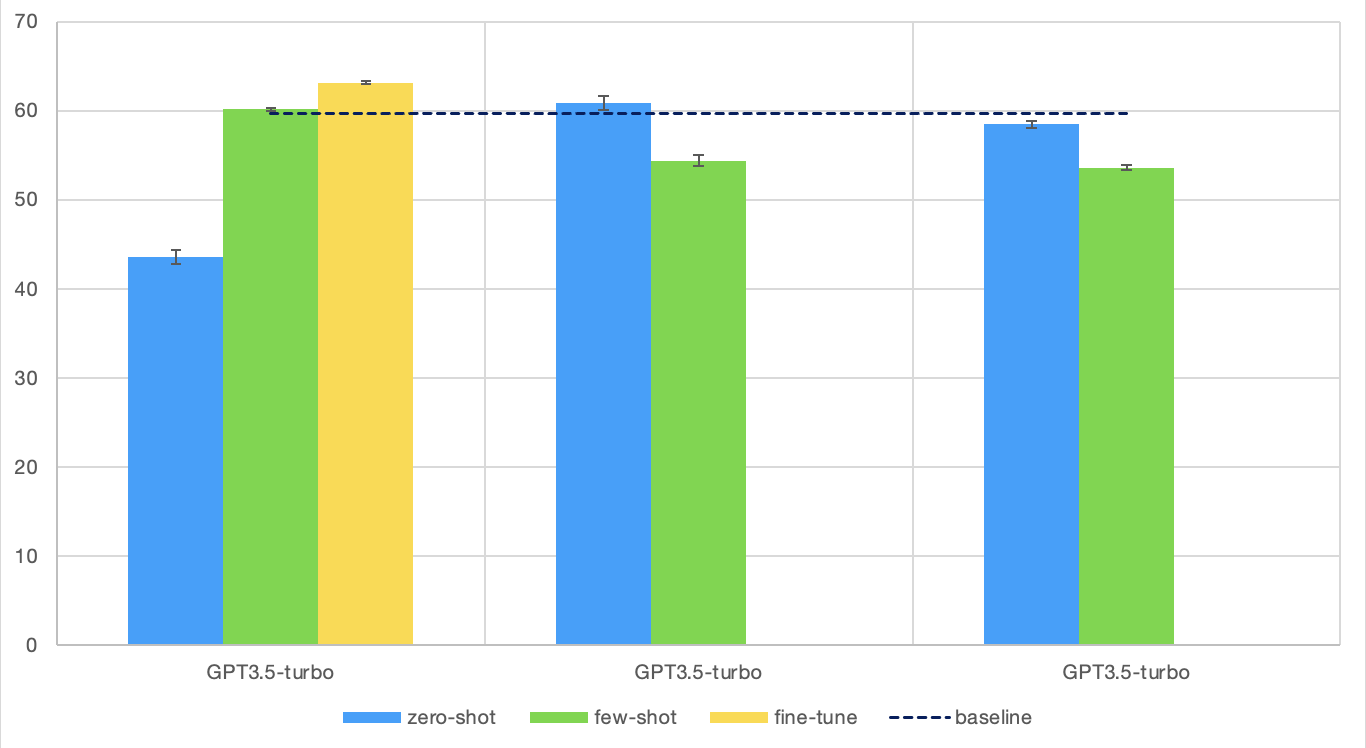
\includegraphics[width=1\textwidth]{figures/ner-measeval-all.png} 
  \caption{Comparison scores for properties extraction NER generation. The scores are the aggregations of the micro average F1 scores. The evaluation scores are calculated using soft matching with a threshold of 0.9 similarity. The error bars are calculated over the standard deviation of three independent runs.}
  \label{fig:ner-measeval-all}
\end{figure}

Surprisingly, none of the models managed to surpass grobid-quantities in zero-shot generation, as illustrated in Figure~\ref{fig:ner-measeval-all}. This outcome is unexpected given that a) the expression of properties does not adhere to a specific domain (aside from potential variations in frequency distribution), and b) quantities and measurements are likely prevalent in the extensive text corpus used to pre-train the OpenAI models.

In the case of few-shot generation (Figure~\ref{fig:ner-measeval-all}), there was a modest improvement observed only for GPT4 and GPT4-Turbo, resulting in a gain ranging from 2\% to 5\% in F1-score. However, this improvement is not substantial. We posit that the hints provided to the language models (LLMs) may introduce bias, and when these hints are incorrect or incomplete, the LLMs struggle to guide the generation effectively, impacting the quality of the output results.
Notably, the fine-tuned model (Figure~\ref{fig:ner-measeval-all}) appears to exhibit a slight enhancement compared to zero-shot, few-shot, and the baseline. Interestingly, in this specific instance where both the baseline and fine-tuned models are trained and evaluated on the same data, the LLM demonstrates an approximate 3\% increase in F1-score.

\subsubsection{Extraction of materials expressions}
\label{sec:results-ner-materials}
The evaluation of material expressions was performed using the validation partition of the SuperMat~\cite{lfoppiano2021supermat} dataset, composed of 32 articles.

\begin{figure}[htbp]
  \centering
  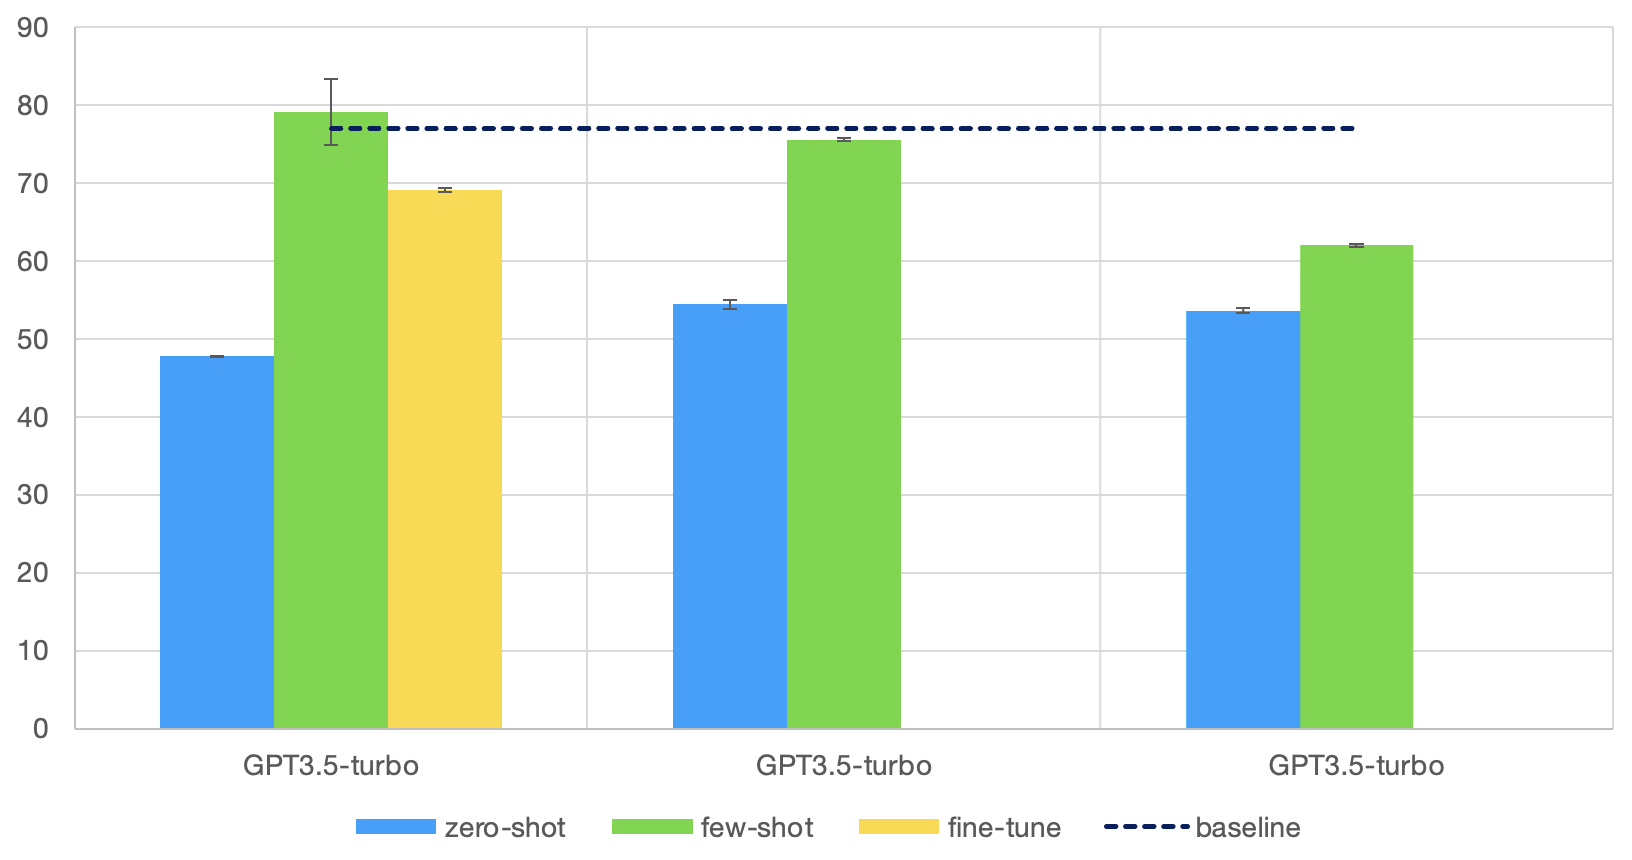
\includegraphics[width=1\textwidth]{figures/ner-supermat-all.png} 
  \caption{Comparison scores for the NER on materials extraction of the three models. The metrics are the aggregations of the micro average F1-scores, calculated using formulas matching. The error bars are calculated over the standard deviation of three independent runs.}
  \label{fig:ner-materials-all}
\end{figure}

In zero-shot generation (Figure~\ref{fig:ner-materials-all}), both GPT4 and GPT4-Turbo achieved comparable F1-scores, hovering around 60\%. Notably, all language models (LLMs) scored more than 10\% lower compared to the baseline~\cite{lfoppiano2023automatic}. This disparity is anticipated, considering that material expressions may involve extensive sequences and encompass multiple pieces of information that are not easily conveyed in the prompt.

Few-shot generation (Figure~\ref{fig:ner-materials-all}) yielded improved results, with GPT3.5-turbo and GPT4 slightly surpassing the baseline. The introduction of hints in the prompt indeed enhances performance, but, as previously discussed, it appears to strongly influence the LLMs. In essence, the LLMs struggle to mitigate the impact of invalid hints that may be provided.

Equally unexpected, fine-tuning did not outperform few-shot generation. This outcome suggests that the additional training did not significantly enhance the LLMs' ability to handle material expressions.

\subsection{Relation extraction}
\label{sec:results-re}

The evaluation of relation extraction employed the entire SuperMat dataset, and the results are depicted in Figure~\ref{fig:re-eval-all}, where the effects of shuffling are compared across different models. Figure~\ref{fig:re-eval-shuffled-all} specifically contrasts the shuffled version of each model and extraction type.

In the context of zero-shot generation (Figure~\ref{fig:re-eval-shuffled-all}), GPT3.5-turbo exhibited the most notable disparity between the shuffled and non-shuffled approaches. This suggests that the generation process merely connects entities of different classes in a sequential manner rather than adhering to a specific contextual reasoning. In contrast, both GPT4 and GPT4-turbo displayed much lower differences in performance under shuffling conditions.

\begin{figure}[htbp]
  \centering
  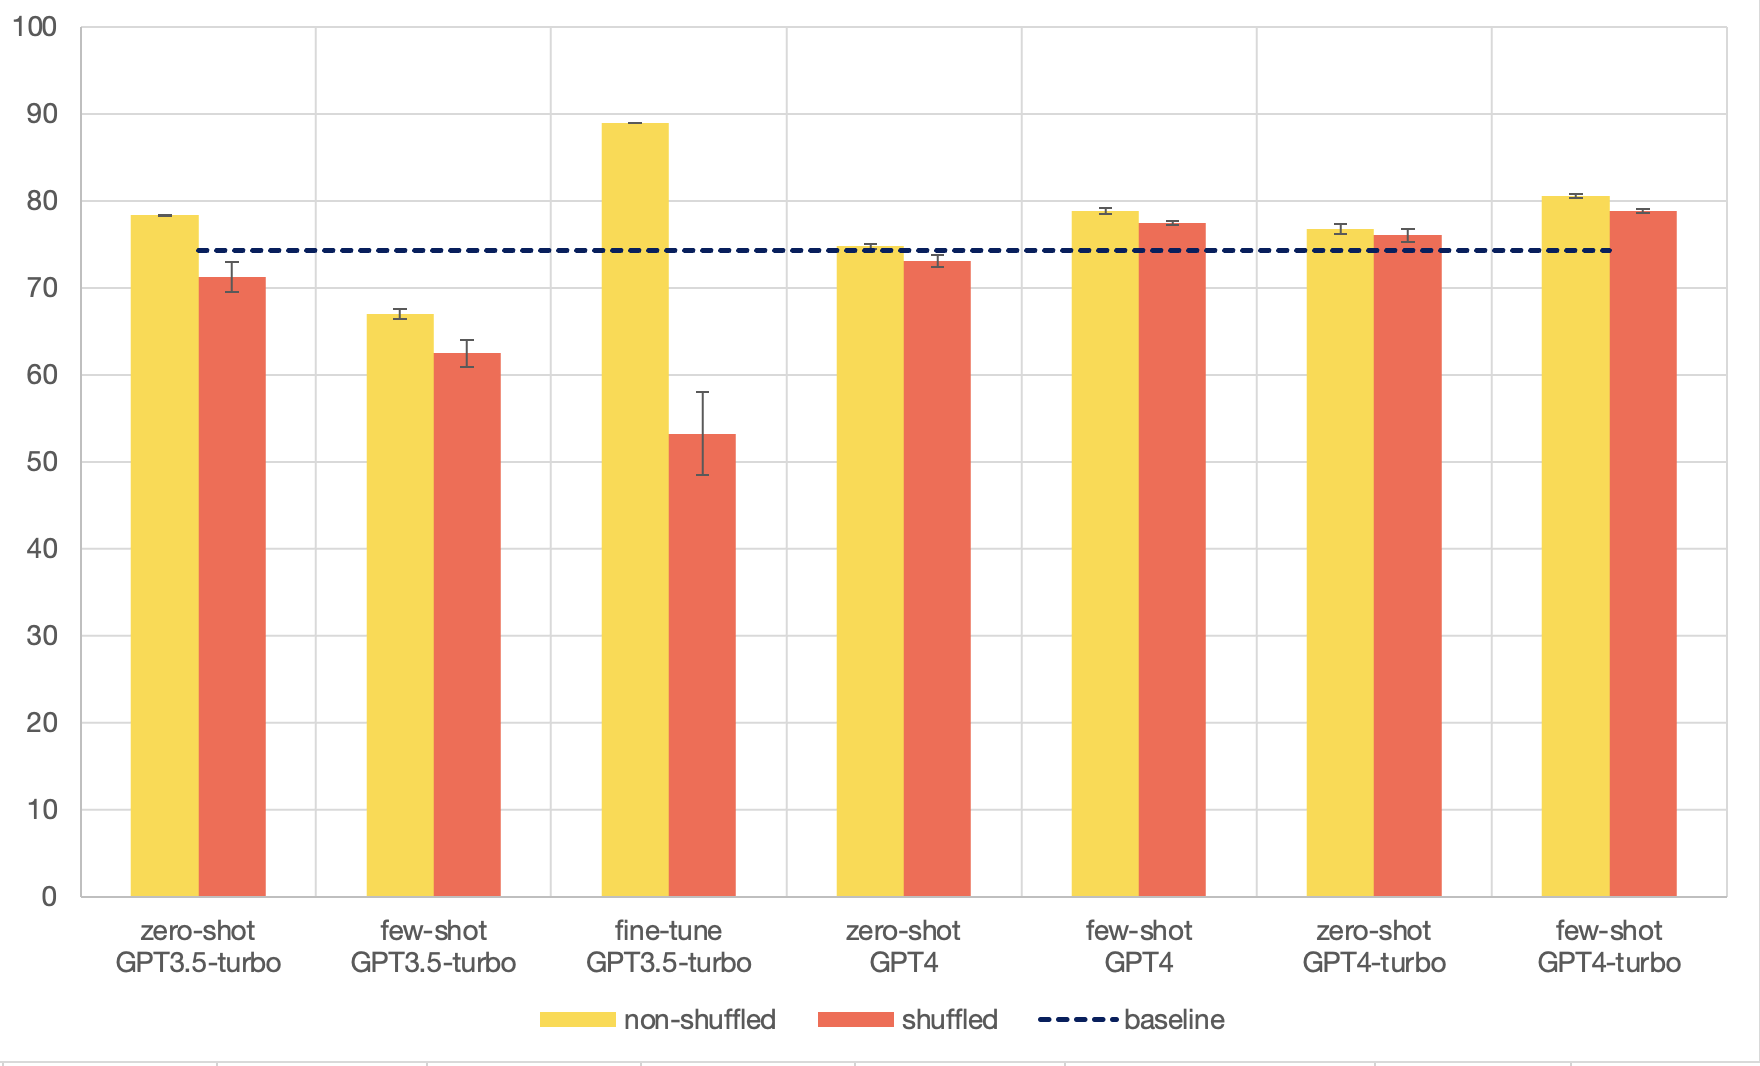
\includegraphics[width=1\textwidth]{figures/re-eval-all.png} 
  \caption{Comparison of the scores of the shuffled extraction using zero-shot, few-shot and fine-tuned of the three models for RE on materials and properties. The metrics are the aggregated micro average F1-scores calculated using strict matching. The error bars are calculated over the standard deviation of three independent runs.}
  \label{fig:re-eval-all}
\end{figure}

Few-shot generation yielded improved scores across all models, showcasing a notable increase in F1-score ranging from 3 to 10\%. These enhancements were achieved by incorporating additional examples in each prompt. Among the models, both GPT4-turbo and GPT4 achieved the highest performance, each attaining around 80\% F1-score.

However, it's noteworthy that the fine-tuned model appears to exhibit reduced flexibility, as evidenced by a slight decrease in F1 score during the shuffled evaluation when compared to the base model.


\begin{figure}[htbp]
  \centering
  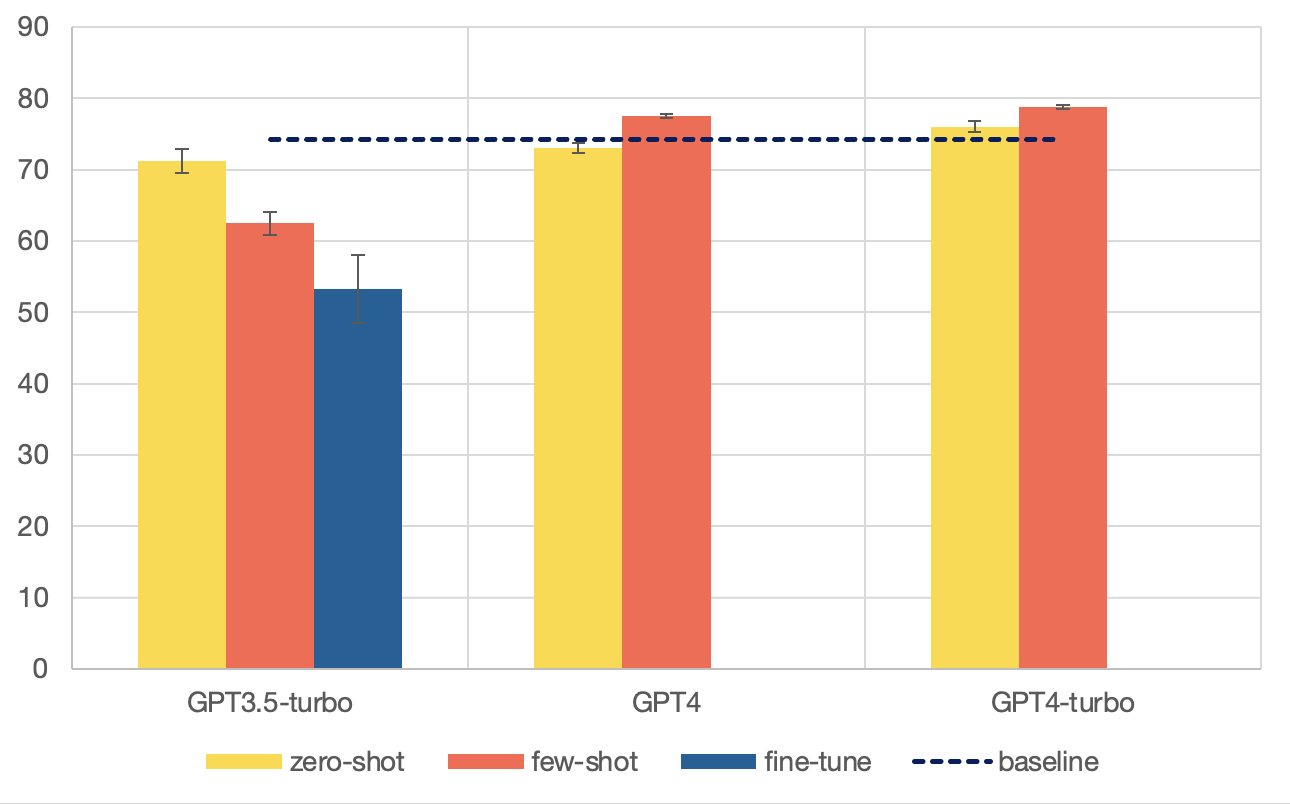
\includegraphics[width=1\textwidth]{figures/re-eval-shuffled-all.png} 
  \caption{Overview evaluation on the effect of shuffling the entities in RE on materials and properties. The metrics are the aggregated micro average F1-scores calculated using strict matching. The error bars are calculated over the standard deviation of three independent runs.}
  \label{fig:re-eval-shuffled-all}
\end{figure}

\section{Conclusion}

When it comes to entity extraction (NER), Large Language Models (LLMs) appear to underperform significantly compared to smaller LMs in both material and property extraction. This finding is particularly surprising since these expressions are not confined to a specific domain.

In material extraction, fine-tuning failed to surpass the baseline, and the same holds true for few-shot generation. Our results suggest that, for material expressions, small specialised models remain the most accurate choice.

For property extraction, zero-shot generation performs on par with the baseline for GPT-4 and GPT-4 Turbo. Few-shot and fine-tuning, on the other hand, outperform the baseline by a marginal increase in points.

The scenario improves for relation extraction:
\begin{enumerate}
\item Few-shot generation, with two examples, demonstrates a significant improvement over the baseline.
\item GPT-4 Turbo exhibits enhanced reasoning capabilities compared to GPT-4 and GPT-3.5 Turbo.
\item GPT-3.5 Turbo performs poorly in both zero-shot and few-shot generation.
\item Fine-tuned GPT-3.5 Turbo shows a substantial score decrease when entities are shuffled, aligning with previous observations.
\end{enumerate}
    
Fine-tuning, overall, does not appear to address all the challenges in both tasks and may struggle to learn to output a valid JSON format.

In conclusion, GPT-4 and GPT-4 Turbo showcase effective reasoning capabilities for relating concepts and extracting relations accurately. However, for the extraction of complex entities such as materials, we find that training small specialised models remains a more effective approach.

\bibliography{references}
\bibliographystyle{unsrt}


\clearpage

\appendix


\section{Full evaluation results}

\subsection{NER for properties extraction}

\subsubsection{Zero-shot prompting}
\begin{table}[htbp]
\small
  \centering
  \caption{Performance Metrics for GPT-3.5-turbo NER in properties extraction, zero-shot prompting. P: Precision, R: Recall, F1: harmonic average of P and R, Supp: Support, number of extracted entities.}
  \begin{tabular}{lccccc}
    \toprule
    \textbf{Run} & \textbf{Matching} & \textbf{P} & \textbf{R} & \textbf{F1} & \textbf{Supp} \\
    \midrule
    \multirow{2}{*}{Run1} & Soft matching & 42.73 & 14.49 & 21.64 & 564 \\
    & Sentence BERT & 45.39 & 15.39 & 22.99 & 564 \\
    \midrule
    \multirow{2}{*}{Run2} & Soft matching & 41.81 & 13.35 & 20.24 & 531 \\
    & Sentence BERT & 45.01 & 14.37 & 21.79 & 531 \\
    \midrule
    \multirow{2}{*}{Run3} & Soft matching & 42.86 & 14.61 & 21.79 & 567 \\
    & Sentence BERT & 45.86 & 15.63 & 23.32 & 567 \\
    \midrule
    \multicolumn{2}{l}{\textbf{Mean and Standard deviation of F1 score}} & & & & \\
    \midrule
    \textbf{Matching} & \textbf{Avg.} & $\sigma\textsuperscript{2}$ & & & \textbf{Avg. Supp}\\
    Soft matching & 21.22 & 0.85 & & & 554 \\
    Sentence BERT & 22.7 & 0.80 & & & \\
    \bottomrule
  \end{tabular}
\end{table}


\begin{table}[htbp]
\small
  \centering
  \caption{Performance Metrics for GPT-4 NER in properties extraction, zero-shot prompting. P: Precision, R: Recall, F1: harmonic average of P and R, Supp: Support, number of extracted entities.}
  \begin{tabular}{lccccc}
    \toprule
    \textbf{Run} & \textbf{Matching} & \textbf{P} & \textbf{R} & \textbf{F1} & \textbf{Supp} \\
    \midrule
    \multirow{2}{*}{Run1} & Soft matching & 61.43 & 56.70 & 58.97 & 1535 \\
    & Sentence BERT & 65.08 & 60.07 & 62.48 & 1535 \\
    \midrule
    \multirow{2}{*}{Run2} & Soft matching & 63.23 & 57.19 & 60.06 & 1504 \\
    & Sentence BERT & 66.42 & 60.07 & 63.09 & 1504 \\
    \midrule
    \multirow{2}{*}{Run3} & Soft matching & 62.83 & 56.52 & 59.51 & 1496 \\
    & Sentence BERT & 66.11 & 59.47 & 62.61 & 1496 \\
    \midrule
    \multicolumn{2}{l}{\textbf{Mean and Standard deviation of F1 score}} & & & & \\
    \midrule
    \textbf{Matching} & \textbf{Avg.} & $\sigma\textsuperscript{2}$ & & & \textbf{Avg. Supp}\\
    Soft matching & 59.51 & 0.54 & & & 1511 \\
    Sentence BERT & 62.72 & 0.32 & & & \\
    \bottomrule
  \end{tabular}
\end{table}


\begin{table}[htbp]
\small
  \centering
  \caption{Performance Metrics for GPT4-turbo NER in properties extraction, zero-shot prompting. P: Precision, R: Recall, F1: harmonic average of P and R, Supp: Support, number of extracted entities.}
  \begin{tabular}{lccccc}
    \toprule
    \textbf{Run} & \textbf{Matching} & \textbf{P} & \textbf{R} & \textbf{F1} & \textbf{Supp} \\
    \midrule
    \multirow{2}{*}{Run1} & Soft matching & 59.60 & 54.30 & 56.83 & 1515 \\
    & Sentence BERT & 62.90 & 57.31 & 59.97 & 1515 \\
    \midrule        
    \multirow{2}{*}{Run2} & Soft matching & 60.34 & 55.44 & 57.79 & 1528 \\
    & Sentence BERT & 63.87 & 58.69 & 61.17 & 1528 \\
    \midrule        
    \multirow{2}{*}{Run3} & Soft matching & 60.05 & 54.60 & 57.20 & 1512 \\    
    & Sentence BERT & 63.96 & 58.15 & 60.91 & 1512 \\
    \midrule
    \multicolumn{2}{l}{\textbf{Mean and Standard deviation of F1 score}} & & & & \\
    \midrule
    \textbf{Matching} & \textbf{Avg.} & $\sigma\textsuperscript{2}$ & & & \textbf{Avg. Supp}\\
    Soft matching & 57.27 & 0.48 & & & 1518 \\
    Sentence BERT & 60.68 & 0.63 & & & \\
    \bottomrule
  \end{tabular}
\end{table}

\clearpage
\subsubsection{Few-shot prompting }

\begin{table}[htbp]
\small
  \centering
  \caption{Performance Metrics for GPT-3.5-turbo NER in properties extraction, few-shot prompting. P: Precision, R: Recall, F1: harmonic average of P and R, Supp: Support, number of extracted entities.}
  \begin{tabular}{lccccc}
    \toprule
    \textbf{Run} & \textbf{Matching} & \textbf{P} & \textbf{R} & \textbf{F1} & \textbf{Supp} \\
    \midrule
    \multirow{2}{*}{Run1} & Soft matching & 60.98 & 57.79 & 59.34 & 1576 \\
    & Sentence BERT & 64.85 & 61.46 & 63.11 & 1576 \\    
    \midrule
    \multirow{2}{*}{Run2} & Soft matching & 60.99 & 57.73 & 59.31 & 1574 \\
    & Sentence BERT & 64.55 & 61.09 & 62.77 & 1574 \\
    \midrule
    \multirow{2}{*}{Run3} & Soft matching & 60.72 & 57.55 & 59.09 & 1576 \\
    & Sentence BERT & 64.28 & 60.91 & 62.55 & 1576 \\
    \midrule
    \multicolumn{2}{l}{\textbf{Mean and Standard deviation of F1 score}} & & & & \\
    \midrule
    \textbf{Matching} & \textbf{Avg.} & $\sigma\textsuperscript{2}$ & & & \textbf{Avg. Supp}\\
    Soft matching & 59.24 & 0.13 & & & 1575 \\
    Sentence BERT & 62.81 & 0.28 & & & \\
    \bottomrule
  \end{tabular}
\end{table}

\begin{table}[htbp]
\small
  \centering
  \caption{Performance Metrics for GPT-4 NER in properties extraction, few-shot prompting. P: Precision, R: Recall, F1: harmonic average of P and R, Supp: Support, number of extracted entities.}
  \begin{tabular}{lccccc}
    \toprule
    \textbf{Run} & \textbf{Matching} & \textbf{P} & \textbf{R} & \textbf{F1} & \textbf{Supp} \\
    \midrule
    \multirow{2}{*}{Run1} & Soft matching & 62.01 & 60.85 & 61.43 & 1632 \\
    & Sentence BERT & 65.56 & 64.34 & 64.95 & 1632 \\
    \midrule    
    \multirow{2}{*}{Run2} & Soft matching & 62.15 & 60.91 & 61.52 & 1630 \\
    & Sentence BERT & 65.52 & 64.22 & 64.86 & 1630 \\
    \midrule    
    \multirow{2}{*}{Run3} & Soft matching & 62.41 & 61.09 & 61.74 & 1628 \\
    & Sentence BERT & 65.6 & 64.22 & 64.9 & 1628 \\
    \midrule    
    \multicolumn{2}{l}{\textbf{Mean and Standard deviation of F1 score}} & & & & \\
    \midrule
    \textbf{Matching} & \textbf{Avg.} & $\sigma\textsuperscript{2}$ & & & \textbf{Avg. Supp}\\
    Soft matching & 61.56 & 0.16 & & & 1630 \\
    Sentence BERT & 64.9 & 0.04 & & & \\
    \bottomrule
  \end{tabular}
\end{table}

\begin{table}[htbp]
\small
  \centering
  \caption{Performance Metrics for GPT-4-turbo NER in properties extraction, few-shot prompting. P: Precision, R: Recall, F1: harmonic average of P and R, Supp: Support, number of extracted entities.}
  \begin{tabular}{lccccc}
    \toprule
    \textbf{Run} & \textbf{Matching} & \textbf{P} & \textbf{R} & \textbf{F1} & \textbf{Supp} \\
    \midrule
    \multirow{2}{*}{Run1} & Soft matching & 62.18 & 62 & 62.09 & 1652 \\
    & Sentence BERT & 65.8 & 65.6 & 65.7 & 1652 \\
    \midrule    
    \multirow{2}{*}{Run2} & Soft matching & 62.42 & 62.24 & 62.33 & 1658 \\
    & Sentence BERT & 66.1 & 65.9 & 66 & 1658 \\
    \midrule    
    \multirow{2}{*}{Run3} & Soft matching & 62.48 & 62.78 & 62.63 & 1671 \\
    & Sentence BERT & 65.95 & 66.27 & 66.11 & 1671 \\
    \midrule
    \multicolumn{2}{l}{\textbf{Mean and Standard deviation of F1 score}} & & & & \\
    \midrule
    \textbf{Matching} & \textbf{Avg.} & $\sigma\textsuperscript{2}$ & & & \textbf{Avg. Supp}\\
    Soft matching & 62.35 & 0.27 & & & 1660 \\
    Sentence BERT & 65.93 & 0.21 & & & \\
    \bottomrule
  \end{tabular}
\end{table}

\clearpage
\subsubsection{Fine-tuning}

\begin{table}[htbp]
\small
  \centering
  \caption{Performance Metrics for fine-tuned GPT-3.5-turbo NER in properties extraction. P: Precision, R: Recall, F1: harmonic average of P and R, Supp: Support, number of extracted entities.}
  \begin{tabular}{lccccc}
    \toprule
    \textbf{Run} & \textbf{Matching} & \textbf{P} & \textbf{R} & \textbf{F1} & \textbf{Supp} \\
    \midrule
    \multirow{2}{*}{Run1} & Soft matching & 60.76 & 58.57 & 59.64 & 1603 \\
    & Sentence BERT & 64.38 & 62.06 & 63.2 & 1603 \\
    \midrule
    \multirow{2}{*}{Run2} & Soft matching & 60.85 & 58.69 & 59.75 & 1604 \\
    & Sentence BERT & 64.4 & 62.12 & 63.24 & 1604 \\
    \midrule
    \multirow{2}{*}{Run3} & Soft matching & 60.49 & 58.45 & 59.45 & 1607 \\
    & Sentence BERT & 64.09 & 61.94 & 63 & 1607 \\
    \midrule
    \multicolumn{2}{l}{\textbf{Mean and Standard deviation of F1 score}} & & & & \\
    \midrule
    \textbf{Matching} & \textbf{Avg.} & $\sigma\textsuperscript{2}$ & & & \textbf{Avg. Supp}\\
    Soft matching & 59.61 & 0.15 & & & 1604 \\
    Sentence BERT & 63.14 & 0.12 & & & \\
    \bottomrule
  \end{tabular}
\end{table}

\clearpage
\subsection{NER for Materials extraction}

\subsubsection{Zero-shot}

\begin{table}[htbp]
\small
  \centering
  \caption{Performance Metrics for GPT3.5-turbo NER in materials extraction, zero-shot prompting. P: Precision, R: Recall, F1: harmonic average of P and R, Supp: Support, number of extracted entities.}
  \begin{tabular}{lccccc}
    \toprule
    \textbf{Run} & \textbf{Matching} & \textbf{P} & \textbf{R} & \textbf{F1} & \textbf{Supp} \\
    \midrule
    \multirow{2}{*}{Run1} & Sentence BERT & 37.34 & 22.58 & 28.14 & 1617 \\
    & Formula & 59.49 & 35.97 & 44.83 & 1617 \\
    \midrule
    \multirow{2}{*}{Run2} & Sentence BERT & 37.06 & 22.83 & 28.26 & 1641 \\
    & Formula & 59.21 & 36.48 & 45.15 & 1641 \\
    \midrule
    \multirow{2}{*}{Run3} & Sentence BERT & 37.45 & 22.07 & 27.77 & 1587 \\
    & Formula & 59.74 & 35.2 & 44.3 & 1587 \\
    \midrule
    \multicolumn{2}{l}{\textbf{Mean and Standard deviation of F1 score}} & & & & \\
    \midrule
    \textbf{Matching} & \textbf{Avg.} & $\sigma\textsuperscript{2}$ & & & \textbf{Avg. Supp}\\
    Sentence BERT & 28.05 & 0.25 & & & 1615 \\
    Formula & 44.76 & 0.42 & & & \\
    \bottomrule
  \end{tabular}
\end{table}



\begin{table}[htbp]
\small
  \centering
  \caption{Performance Metrics for GPT-4 NER in materials extraction, zero-shot prompting. P: Precision, R: Recall, F1: harmonic average of P and R, Supp: Support, number of extracted entities.}
  \begin{tabular}{lccccc}
    \toprule
    \textbf{Run} & \textbf{Matching} & \textbf{P} & \textbf{R} & \textbf{F1} & \textbf{Supp} \\
    \midrule
    \multirow{2}{*}{Run1} & Sentence BERT & 49.9 & 31.25 & 38.43 & 1103 \\
    & Formula & 66.4 & 41.58 & 51.14& 1103 \\
    \midrule
    \multirow{2}{*}{Run2} & Sentence BERT & 49.9 & 30.61 & 37.94 & 1097 \\
    & Formula & 66.94 & 41.07 & 50.91 & 1097 \\
    \midrule
    \multirow{2}{*}{Run3} & Sentence BERT & 49.59 & 30.74 & 37.95 & 1108 \\
    & Formula & 66.46 & 41.2 & 50.87 & 1108 \\
    \midrule
    \multicolumn{2}{l}{\textbf{Mean and Standard deviation of F1 score}} & & & & \\
    \midrule
    \textbf{Matching} & \textbf{Avg.} & $\sigma\textsuperscript{2}$ & & & \textbf{Avg. Supp}\\
    Sentence BERT & 38.10 & 0.28 & & & 1102 \\
    Formula & 50.97 & 0.14 & & & \\
    \bottomrule
  \end{tabular}
\end{table}

\begin{table}[htbp]
\small
  \centering
  \caption{Performance Metrics for GPT4-turbo NER in properties extraction, zero-shot prompting. P: Precision, R: Recall, F1: harmonic average of P and R, Supp: Support, number of extracted entities.}
  \begin{tabular}{lccccc}
    \toprule
    \textbf{Run} & \textbf{Matching} & \textbf{P} & \textbf{R} & \textbf{F1} & \textbf{Supp} \\
    \midrule
    \multirow{2}{*}{Run1} & Sentence BERT & 45.53 & 22.07 & 29.73 & 883 \\
    & Formula & 70.53 & 34.18 & 46.05 & 883 \\
    \midrule
    \multirow{2}{*}{Run2} & Sentence BERT & 46.67 & 22.32 & 30.2 & 873 \\
    & Formula & 70.67 & 33.8 & 45.73 & 873 \\
    \midrule
    \multirow{2}{*}{Run3} & Sentence BERT & 46.74 & 22.83 & 30.68 & 878 \\
    & Formula & 70.5 & 34.44 & 46.27 & 878 \\
    \midrule
    \multicolumn{2}{l}{\textbf{Mean and Standard deviation of F1 score}} & & & & \\
    \midrule
    \textbf{Matching} & \textbf{Avg.} & $\sigma\textsuperscript{2}$ & & & \textbf{Avg. Supp}\\
    Sentence BERT & 45.98 & 0.56 & & & 878 \\
    Formula & 53.60 & 0.30 & & & \\
    \bottomrule
  \end{tabular}
\end{table}


\clearpage
\subsubsection{Few-shot}

\begin{table}[htbp]
\small
  \centering
  \caption{Performance Metrics for GPT3.5-turbo NER in materials extraction, few-shot prompting. P: Precision, R: Recall, F1: harmonic average of P and R, Supp: Support, number of extracted entities.}
  \begin{tabular}{lccccc}
    \toprule
    \textbf{Run} & \textbf{Matching} & \textbf{P} & \textbf{R} & \textbf{F1} & \textbf{Supp} \\
    \midrule
    \multirow{2}{*}{Run1} & Sentence BERT & 71.58 & 69.39 & 70.47 & 1887 \\
    & Formula & 75.79 & 73.47 & 74.61 & 1887 \\
    \midrule
    \multirow{2}{*}{Run2} & Sentence BERT & 78.73 & 88.78 & 83.45 & 2495 \\
    & Formula & 78.39 & 88.39 & 83.09 & 2495 \\
    \midrule
    \multirow{2}{*}{Run3} & Sentence BERT & 78.85 & 88.9 & 83.57 & 2448 \\
    & Formula & 78.73 & 88.78 & 83.45 & 2448 \\
    \midrule
    \multicolumn{2}{l}{\textbf{Mean and Standard deviation of F1 score}} & & & & \\
    \midrule
    \textbf{Matching} & \textbf{Avg.} & $\sigma\textsuperscript{2}$ & & & \textbf{Avg. Supp}\\
    Sentence BERT & 79.16 & 7.5 & & & 2276 \\
    Formula & 80.38 & 4.82 & & & \\
    \bottomrule
  \end{tabular}
\end{table}


\begin{table}[htbp]
\small
  \centering
  \caption{Performance Metrics for GPT-4 NER in materials extraction, few-shot prompting. P: Precision, R: Recall, F1: harmonic average of P and R, Supp: Support, number of extracted entities.}
  \begin{tabular}{lccccc}
    \toprule
    \textbf{Run} & \textbf{Matching} & \textbf{P} & \textbf{R} & \textbf{F1} & \textbf{Supp} \\
    \midrule
    \multirow{2}{*}{Run1} & Sentence BERT & 75.87 & 75 & 75.43 & 1402 \\
    & Formula & 77.16 & 76.28 & 76.72 & 1412 \\
    \midrule
    \multirow{2}{*}{Run2} & Sentence BERT & 70.67 & 82.65 & 76.19 & 1402 \\
    & Formula & 70.99 & 83.04 & 76.54 & 1854 \\
    \midrule
    \multirow{2}{*}{Run3} & Sentence BERT & 70.99 & 83.04 & 76.54 & 1402 \\
    & Formula & 72.09 & 83.67 & 77.45 & 1826 \\
    \midrule
    \multicolumn{2}{l}{\textbf{Mean and Standard deviation of F1 score}} & & & & \\
    \midrule
    \textbf{Matching} & \textbf{Avg.} & $\sigma\textsuperscript{2}$ & & & \textbf{Avg. Supp}\\
    Sentence BERT & 76.35 & 1.02 & & & 1402 \\
    Formula & 76.90 & 0.48 & & & \\
    \bottomrule
  \end{tabular}
\end{table}


\begin{table}[htbp]
\small
  \centering
  \caption{Performance Metrics for GPT4-turbo NER in materials extraction, few-shot prompting. P: Precision, R: Recall, F1: harmonic average of P and R, Supp: Support, number of extracted entities.}
  \begin{tabular}{lccccc}
    \toprule
    \textbf{Run} & \textbf{Matching} & \textbf{P} & \textbf{R} & \textbf{F1} & \textbf{Supp} \\
    \midrule
    \multirow{2}{*}{Run1} & Sentence BERT & 54.78 & 59.95 & 57.25 & 1735 \\
    & Formula & 60.26 & 65.94 & 62.97 & 1735 \\
    \midrule
    \multirow{2}{*}{Run2} & Sentence BERT & 55.54 & 59.44 & 57.42 & 1707 \\
    & Formula & 60.91 & 65.18 & 62.97 & 1707 \\
    \midrule
    \multirow{2}{*}{Run3} & Sentence BERT & 55.81 & 60.08 & 57.86 & 1707 \\
    & Formula & 61.02 & 65.69 & 63.27 & 1707 \\
    \midrule
    \multicolumn{2}{l}{\textbf{Mean and Standard deviation of F1 score}} & & & & \\
    \midrule
    \textbf{Matching} & \textbf{Avg.} & $\sigma\textsuperscript{2}$ & & & \textbf{Avg. Supp}\\
    Sentence BERT & 57.51 & 0.31 & & & 1716 \\
    Formula & 63.07 & 0.17 & & & \\
    \bottomrule
  \end{tabular}
\end{table}

\clearpage
\subsubsection{Fine-tuning}

\begin{table}[htbp]
\small
  \centering
  \caption{Performance Metrics for the fine-tuned GPT3.5-turbo NER in materials extraction. P: Precision, R: Recall, F1: harmonic average of P and R, Supp: Support, number of extracted entities.}
  \begin{tabular}{lccccc}
    \toprule
    \textbf{Run} & \textbf{Matching} & \textbf{P} & \textbf{R} & \textbf{F1} & \textbf{Supp} \\
    \midrule
    \multirow{2}{*}{Run1} & Sentence BERT & 61.02 & 65.69 & 63.27 & 1429 \\
    & Formula & 61.02 & 65.69 & 63.27 & 1429 \\
    \midrule
    \multirow{2}{*}{Run2} & Sentence BERT & 72.24 & 67.73 & 69.91 & 1429 \\
    & Formula & 80.14 & 75.13 & 77.55 & 1429 \\
    \midrule
    \multirow{2}{*}{Run3} & Sentence BERT & 72.17 & 67.47 & 69.74 & 1432 \\
    & Formula & 80.08 & 74.87 & 77.39 & 1432 \\
    \midrule
    \multicolumn{2}{l}{\textbf{Mean and Standard deviation of F1 score}} & & & & \\
    \midrule
    \textbf{Matching} & \textbf{Avg.} & $\sigma\textsuperscript{2}$ & & & \textbf{Avg. Supp}\\
    Sentence BERT & 69.75 & 0.15 & & & 1430 \\
    Formula & 77.43 & 0.09 & & & \\
    \bottomrule
  \end{tabular}
\end{table}

\clearpage
\subsection{RE for Materials-Properties extraction}

\subsubsection{Zero-shot}

\begin{table}[htbp]
  \small
  \centering
  \caption{Performance Metrics for the GPT3.5-turbo model on RE in materials-properties extraction. In this run, entities are not shuffled when included in the prompt. P: Precision, R: Recall, F1: harmonic average of P and R, Supp: Support, number of extracted entities.}
  \begin{tabular}{lccccc}
    \toprule
    \textbf{Run} & \textbf{Matching} & \textbf{P} & \textbf{R} & \textbf{F1} & \textbf{Supp} \\
    \midrule
    \multirow{2}{*}{Run1} & Strict matching & 80.41 & 65.7 & 72.32 & 934 \\
    & Soft matching & 80.73 & 65.97 & 72.6 & 934 \\
    \midrule
    \multirow{2}{*}{Run2} & Strict matching & 80.41 & 54.59 & 65.03 & 776 \\
    & Soft matching & 80.8 & 54.86 & 65.35 & 776 \\
    \midrule
    \multirow{2}{*}{Run3} & Strict matching & 80.25 & 55.47 & 65.6 & 790 \\
    & Soft matching & 80.51 & 55.64 & 65.8 & 790 \\
    \midrule
    \multicolumn{2}{l}{\textbf{Mean and Standard deviation of F1 score}} & & & & \\
    \midrule
    \textbf{Matching} & \textbf{Avg.} & $\sigma\textsuperscript{2}$ & & & \textbf{Avg. Supp}\\
    Strict matching & 67.65 & 4.05 & & & 833 \\
    Soft matching & 67.91 & 4.06 & & & \\
    \bottomrule
  \end{tabular}
\end{table}


\begin{table}[htbp]
    \small
    \centering
    \caption{Performance Metrics for the GPT3.5-turbo model on RE in materials-properties extraction. In this run, entities are shuffled to make it more challenging for the LLM. P: Precision, R: Recall, F1: harmonic average of P and R, Supp: Support, number of extracted entities.}
    \begin{tabular}{lccccc}
        \toprule
        \textbf{Run} & \textbf{Matching} & \textbf{P} & \textbf{R} & \textbf{F1} & \textbf{Supp} \\
        \midrule
        \multirow{2}{*}{Run1} & Strict matching & 76.12 & 60.8 & 67.61 & 913 \\
        & Soft matching & 76.67 & 61.24 & 68.09 & 913 \\
        \midrule
        \multirow{2}{*}{Run2} & Strict matching & 72.08 & 48.56 & 58.02 & 770 \\
        & Soft matching & 73.12 & 49.26 & 58.86 & 770 \\
        \midrule
        \multirow{2}{*}{Run3} & Strict matching & 74.9 & 49.61 & 59.68 & 757 \\
        & Soft matching & 75.17 & 49.78 & 59.89 & 757 \\
        \midrule
        \multicolumn{2}{l}{\textbf{Mean and Standard deviation of F1 score}} & & & & \\
        \midrule
        \textbf{Matching} & \textbf{Avg.} & $\sigma\textsuperscript{2}$ & & & \textbf{Avg. Supp}\\
        Strict matching & 61.77 & 5.12 & & & 813 \\
        Soft matching & 62.28 & 5.05 & & \\
        \bottomrule
    \end{tabular}
\end{table}

%GPT4

\begin{table}[htbp]
    \small
    \centering
    \caption{Performance Metrics for the GPT-4 model on RE in materials-properties extraction. In this run, entities are not shuffled when added to the prompt. P: Precision, R: Recall, F1: harmonic average of P and R, Supp: Support, number of extracted entities.}
    \begin{tabular}{lccccc}
        \toprule
        \textbf{Run} & \textbf{Matching} & \textbf{P} & \textbf{R} & \textbf{F1} & \textbf{Supp} \\
        \midrule
        \multirow{2}{*}{Run1} & Strict matching & 76.87 & 66.58 & 71.35 & 990 \\
        & Soft matching & 77.47 & 67.1 & 71.92 & 990 \\
        \midrule
        \multirow{2}{*}{Run2} & Strict matching & 76.4 & 67.98 & 71.94 & 1017 \\
        & Soft matching & 76.5 & 68.07 & 72.04 & 1017 \\
        \midrule
        \multirow{2}{*}{Run3} & Strict matching & 76.8 & 68.07 & 72.17 & 1013 \\
        & Soft matching & 76.9 & 68.15 & 72.26 & 1013 \\
        \midrule
        \multicolumn{2}{l}{\textbf{Mean and Standard deviation of F1 score}} & & & & \\
        \midrule
        \textbf{Matching} & \textbf{Avg.} & $\sigma\textsuperscript{2}$ & & & \textbf{Avg. Supp}\\
        Strict matching & 71.82 & 0.42 & & & 1006 \\
        Soft matching   & 72.07 & 0.17 & & \\
        \bottomrule
    \end{tabular}
\end{table}


\begin{table}[htbp]
    \small
    \centering
    \caption{Performance Metrics for the GPT4 model on RE in materials-properties extraction. In this run, entities are shuffled to make it more challenging for the LLM. P: Precision, R: Recall, F1: harmonic average of P and R, Supp: Support, number of extracted entities.}
    \begin{tabular}{lccccc}
        \toprule
        \textbf{Run} & \textbf{Matching} & \textbf{P} & \textbf{R} & \textbf{F1} & \textbf{Supp} \\
        \midrule
        \multirow{2}{*}{Run1} & Strict matching & 75.86 & 65.97 & 70.57 & 994 \\
        & Soft matching & 76.16 & 66.23 & 70.85 & 994 \\
        \midrule
        \multirow{2}{*}{Run2} & Strict matching & 74.06 & 65.44 & 69.48 & 1010 \\
        & Soft matching & 74.06 & 65.44 & 69.48 & 1010 \\
        \midrule
        \multirow{2}{*}{Run3} & Strict matching & 75.37 & 66.4 & 70.6 & 1007 \\
        & Soft matching & 75.57 & 66.58 & 70.79 & 1007 \\
        \midrule
        \multicolumn{2}{l}{\textbf{Mean and Standard deviation of F1 score}} & & & & \\
        \midrule
        \textbf{Matching} & \textbf{Avg.} & $\sigma\textsuperscript{2}$ & & & \textbf{Avg. Supp}\\
        Strict matching & 70.21 & 0.63 & & & 1003 \\
        Soft matching   & 70.37 & 0.77 & & \\
        \bottomrule
    \end{tabular}
\end{table}


% GPT4-turbo
\begin{table}[htbp]
    \small
    \centering
    \caption{Performance Metrics for the GPT4-turbo model on RE in materials-properties extraction. In this run, entities are not shuffled when added to the prompt. P: Precision, R: Recall, F1: harmonic average of P and R, Supp: Support, number of extracted entities.}
    \begin{tabular}{lccccc}
        \toprule
        \textbf{Run} & \textbf{Matching} & \textbf{P} & \textbf{R} & \textbf{F1} & \textbf{Supp} \\
        \midrule
        \multirow{2}{*}{Run1} & Strict matching & 79.8 & 69.12 & 74.07 & 990 \\
        & Soft matching & 80.61 & 69.82 & 74.82 & 990 \\
        \midrule
        \multirow{2}{*}{Run2} & Strict matching & 80.22 & 69.2 & 74.31 & 986 \\
        & Soft matching & 81.03 & 69.9 & 75.06 & 986 \\
        \midrule
        \multirow{2}{*}{Run3} & Strict matching & 78.87 & 73.65 & 76.17 & 989 \\
        & Soft matching & 79.88 & 69.12 & 74.11 & 989 \\
        \midrule
        \multicolumn{2}{l}{\textbf{Mean and Standard deviation of F1 score}} & & & & \\
        \midrule
        \textbf{Matching} & \textbf{Avg.} & $\sigma\textsuperscript{2}$ & & & \textbf{Avg. Supp}\\
        Strict matching & 73.85	& 0.60 & & & 988 \\
        Soft matching & 74.66 & 0.49 & & \\
        \bottomrule
    \end{tabular}
\end{table}

\begin{table}[htbp]
    \small
    \centering
    \caption{Performance Metrics for the GPT4-turbo model on RE in materials-properties extraction. In this run, entities are shuffled to make it more challenging for the LLM. P: Precision, R: Recall, F1: harmonic average of P and R, Supp: Support, number of extracted entities.}
    \begin{tabular}{lccccc}
        \toprule
        \textbf{Run} & \textbf{Matching} & \textbf{P} & \textbf{R} & \textbf{F1} & \textbf{Supp} \\
        \midrule
        \multirow{2}{*}{Run1} & Strict matching & 80.04 & 67.37 & 73.16 & 962 \\
        & Soft matching & 80.98 & 68.15 & 74.01 & 962 \\
        \midrule
        \multirow{2}{*}{Run2} & Strict matching & 80.71 & 67.72 & 73.64 & 959 \\
        & Soft matching & 81.44 & 68.33 & 74.31 & 959 \\
        \midrule
        \multirow{2}{*}{Run3} & Strict matching & 79.27 & 66.58 & 72.37 & 960 \\
        & Soft matching & 80.21 & 66.58 & 72.37 & 960 \\
        \midrule
        \multicolumn{2}{l}{\textbf{Mean and Standard deviation of F1 score}} & & & & \\
        \midrule
        \textbf{Matching} & \textbf{Avg.} & $\sigma\textsuperscript{2}$ & & & \\
        Strict matching & 76.05 & 0.74 & & & 960 \\
        Soft matching & 76.87 & 0.64 & & & \\
        \bottomrule
    \end{tabular}
\end{table}


\clearpage
\subsubsection{Few-shot}

% gpt3.5-turbo few shot not shuffled 

\begin{table}[htbp]
    \small
    \centering
    \caption{Performance Metrics for the GPT3.5-turbo model on RE in materials-properties extraction. In this run, entities are shuffled to make it more challenging for the LLM. P: Precision, R: Recall, F1: harmonic average of P and R, Supp: Support, number of extracted entities.}
    \begin{tabular}{lccccc}
        \toprule
        \textbf{Run} & \textbf{Matching} & \textbf{P} & \textbf{R} & \textbf{F1} & \textbf{Supp} \\
        \midrule
        \multirow{2}{*}{Run1} & Strict matching & 67.97 & 50.31 & 57.82 & 846 \\
        & Soft matching & 69.27 & 51.27 & 58.92 & 846 \\
        \midrule
        \multirow{2}{*}{Run2} & Strict matching & 68.2 & 50.48 & 58.02 & 846 \\
        & Soft matching & 69.5 & 51.44 & 59.13 & 846 \\
        \midrule
        \multirow{2}{*}{Run3} & Strict matching & 69.23 & 50.39 & 58.33 & 832 \\
        & Soft matching & 71.18 & 51.09 & 59.14 & 832 \\
        \midrule
        \multicolumn{2}{l}{\textbf{Mean and Standard deviation of F1 score}} & & & & \\
        \midrule
        \textbf{Matching} & \textbf{Avg.} & $\sigma\textsuperscript{2}$ & & & \textbf{Avg. Supp}\\
        Strict matching & 58.05 & 0.25 & & & 841 \\
        Soft matching & 59.06 & 0.12 & & & \\
        \bottomrule
    \end{tabular}
\end{table}


% gpt3.5-turbo few shot shuffled 
\begin{table}[htbp]
    \small
    \centering
    \caption{Performance Metrics for the GPT3.5-turbo model on RE in materials-properties extraction. In this run, entities are shuffled to make it more challenging for the LLM. P: Precision, R: Recall, F1: harmonic average of P and R, Supp: Support, number of extracted entities.}
    \begin{tabular}{lccccc}
        \toprule
        \textbf{Run} & \textbf{Matching} & \textbf{P} & \textbf{R} & \textbf{F1} & \textbf{Supp} \\
        \midrule
        \multirow{2}{*}{Run1} & Strict matching & 63.97 & 47.68 & 54.64 & 852 \\
        & Soft matching & 66.08 & 49.26 & 56.44 & 852 \\
        \midrule
        \multirow{2}{*}{Run2} & Strict matching & 66.02 & 47.59 & 55.31 & 824 \\
        & Soft matching & 67.23 & 48.47 & 56.33 & 824 \\
        \midrule
        \multirow{2}{*}{Run3} & Strict matching & 62.24 & 45.14 & 52.33 & 829 \\
        & Soft matching & 63.93 & 46.37 & 53.75 & 829 \\
        \midrule
        \multicolumn{2}{l}{\textbf{Mean and Standard deviation of F1 score}} & & & & \\
        \midrule
        \textbf{Matching} & \textbf{Avg.} & $\sigma\textsuperscript{2}$ & & & \textbf{Avg. Supp}\\
        Strict matching & 54.09 & 1.56 & & & 835 \\
        Soft matching   & 55.50 & 1.52 & & \\
        \bottomrule
    \end{tabular}
\end{table}

% GPT4 few shot not shuffled 
\begin{table}[htbp]
    \small
    \centering
    \caption{Performance Metrics for the GPT4 model on RE in materials-properties extraction. In this run, entities are not shuffled when they are added to the prompt. P: Precision, R: Recall, F1: harmonic average of P and R, Supp: Support, number of extracted entities.}
    \begin{tabular}{lccccc}
        \toprule
        \textbf{Run} & \textbf{Matching} & \textbf{P} & \textbf{R} & \textbf{F1} & \textbf{Supp} \\
        \midrule
        \multirow{2}{*}{Run1} & Strict matching & 80.57 & 71.83 & 75.95 & 1019 \\
        & Soft matching & 80.57 & 71.83 & 75.95 & 1019 \\
        \midrule
        \multirow{2}{*}{Run2} & Strict matching & 81.29 & 72.62 & 76.71 & 1021 \\
        & Soft matching & 81.39 & 72.7  & 76.8 & 1021 \\
        \midrule
        \multirow{2}{*}{Run3} & Strict matching & 80.9 & 72.27 & 76.34 & 1021 \\
        & Soft matching & 80.9 & 72.27 & 76.34 & 1021 \\
        \midrule
        \multicolumn{2}{l}{\textbf{Mean and Standard deviation of F1 score}} & & & & \\
        \midrule
        \textbf{Matching} & \textbf{Avg.} & $\sigma\textsuperscript{2}$ & & & \textbf{Avg. Supp}\\
        Strict matching & 76.33 & 0.38 & & & 1020 \\
        Soft matching & 76.36 & 0.42 & & \\
        \bottomrule
    \end{tabular}
\end{table}

% gpt4 few-shot shuffled 

\begin{table}[htbp]
    \small
    \centering
    \caption{Performance Metrics for the GPT4 model on RE in materials-properties extraction. In this run, entities are shuffled to make the task more challenging for the LLM. P: Precision, R: Recall, F1: harmonic average of P and R, Supp: Support, number of extracted entities.}
    \begin{tabular}{lccccc}
        \toprule
        \textbf{Run} & \textbf{Matching} & \textbf{P} & \textbf{R} & \textbf{F1} & \textbf{Supp} \\
        \midrule
        \multirow{2}{*}{Run1} & Strict matching & 80.57 & 70.17 & 74.5 & 1010 \\
        & Soft matching & 80.57 & 70.25 & 74.59 & 1010 \\
        \midrule
        \multirow{2}{*}{Run2} & Strict matching & 81.29 & 70.87 & 75.03 & 1016 \\
        & Soft matching & 81.39 & 71.13 & 75.31 & 1016 \\
        \midrule
        \multirow{2}{*}{Run3} & Strict matching & 80.9 & 70.6 & 75.07 & 1007 \\
        & Soft matching & 80.9 & 70.6 & 75.07 & 1007 \\
        \midrule
        \multicolumn{2}{l}{\textbf{Mean and Standard deviation of F1 score}} & & & & \\
        \midrule
        \textbf{Matching} & \textbf{Avg.} & $\sigma\textsuperscript{2}$ & & & \textbf{Avg. Supp}\\
        Strict matching & 74.86 & 0.31 & & & 1011 \\
        Soft matching & 74.99 & 0.36 & & \\
        \bottomrule
    \end{tabular}
\end{table}

% GPT4-turbo not shuffled 

\begin{table}[htbp]
    \small
    \centering
    \caption{Performance Metrics for the GPT4-turbo model on RE in materials-properties extraction. In this run, entities are not shuffled when they are added to the prompt. P: Precision, R: Recall, F1: harmonic average of P and R, Supp: Support, number of extracted entities.}
    \begin{tabular}{lccccc}
        \toprule
        \textbf{Run} & \textbf{Matching} & \textbf{P} & \textbf{R} & \textbf{F1} & \textbf{Supp}\\
        \midrule
        \multirow{2}{*}{Run1} & Strict matching & 83.44 & 70.08 & 76.18 & 960 \\
        & Soft matching & 84.69 & 71.13 & 77.32 & 960 \\
        \midrule
        \multirow{2}{*}{Run2} & Strict matching & 84.1 & 70.34 & 76.61 & 956 \\
        & Soft matching & 85.46 & 71.48 & 77.85 & 956 \\
        \midrule
        \multirow{2}{*}{Run3} & Strict matching & 84.01 & 70.34 & 76.57 & 957 \\
        & Soft matching & 85.37 & 71.48 & 77.81 & 957 \\
        \midrule
        \multicolumn{2}{l}{\textbf{Mean and Standard deviation of F-Score}} & & & & \\
        \midrule
        \textbf{Matching} & \textbf{Avg.} & $\sigma\textsuperscript{2}$ & & & \textbf{Avg. Supp}\\
        Strict matching & 76.45 & 0.23 & & & 957 \\
        Soft matching & 77.66 & 0.29 & & \\
        \bottomrule
    \end{tabular}
\end{table}

% GPT4-turbo  shuffled 

\begin{table}[htbp]
    \small
    \centering
    \caption{Performance Metrics for the GPT4-turbo model on RE in materials-properties extraction. In this run, entities are shuffled to make the task more challenging for the LLM. P: Precision, R: Recall, F1: harmonic average of P and R, Supp: Support, number of extracted entities.}
    \begin{tabular}{lccccc}
        \toprule
        \textbf{Run} & \textbf{Matching} & \textbf{P} & \textbf{R} & \textbf{F1} & \textbf{Supp} \\
        \midrule
        \multirow{2}{*}{Run1} & Strict matching & 82.01 & 67.02 & 73.76 & 934 \\
        & Soft matching & 83.51 & 68.24 & 75.11 & 934 \\
        \midrule
        \multirow{2}{*}{Run2} & Strict matching & 84.11 & 69.47 & 76.09 & 944 \\
        & Soft matching & 85.49 & 70.6 & 77.34 & 944 \\
        \midrule
        \multirow{2}{*}{Run3} & Strict matching & 82.31 & 67.98 & 74.46 & 944 \\
        & Soft matching & 84.32 & 69.64 & 76.28 & 944 \\
        \midrule
        \multicolumn{2}{l}{\textbf{Mean and Standard deviation of F-Score}} & & & & \\
        \midrule
        \textbf{Matching} & \textbf{Avg.} & $\sigma\textsuperscript{2}$ & & & \textbf{Avg. Supp}\\
        Strict matching & 74.77 & 1.19 & & & 940 \\
        Soft matching & 76.24 & 1.11 & & \\
        \bottomrule
    \end{tabular}
\end{table}

\clearpage
\subsubsection{Fine-tuning}

\begin{table}[htbp]
    \small
    \centering
    \caption{Performance Metrics for the GPT3.5-turbo model fine-tuned using the strategy "FT.base" on RE in materials-properties extraction. In this run, entities are not shuffled when included in the prompt. P: Precision, R: Recall, F1: harmonic average of P and R, Supp: Support, number of extracted entities.}
    \begin{tabular}{lccccc}
        \toprule
        \textbf{Run} & \textbf{Matching} & \textbf{P} & \textbf{R} & \textbf{F1} & \textbf{Supp} \\
        \midrule
        \multirow{2}{*}{Run1} & Strict matching & 91.06 & 80.00 & 85.17 & 123 \\
        & Soft matching & 93.50 & 82.14 & 87.45 & 123 \\
        \midrule
        \multirow{2}{*}{Run2} & Strict matching & 91.06 & 80.00 & 85.17 & 123 \\
        & Soft matching & 93.50 & 82.14 & 87.45 & 123 \\
        \midrule
        \multirow{2}{*}{Run3} & Strict matching & 91.06 & 80.00 & 85.17 & 123 \\
        & Soft matching & 93.50 & 82.14 & 87.45 & 123 \\
        \midrule
        \multicolumn{2}{l}{\textbf{Mean and Standard deviation of F1 score}} & & & & \\
        \midrule
        \textbf{Matching} & \textbf{Avg.} & $\sigma\textsuperscript{2}$ & & & \textbf{Avg. Supp}\\
        Strict matching & 85.17 & 0 &  & &  123 \\
        Soft matching & 87.45 & 0 & \\
        \bottomrule
    \end{tabular}
\end{table}


\begin{table}[htbp]
    \small
    \centering
    \caption{Performance Metrics for the GPT3.5-turbo model fine-tuned using the strategy "FT.base" on RE in materials-properties extraction. In this run, entities are shuffled to make it more challenging for the LLM. P: Precision, R: Recall, F1: harmonic average of P and R, Supp: Support, number of extracted entities.}
    \begin{tabular}{lccccc}
        \toprule
        \textbf{Run} & \textbf{Matching} & \textbf{P} & \textbf{R} & \textbf{F1} & \textbf{Supp} \\
        \midrule
        \multirow{2}{*}{Run1} & Strict matching & 92.68 & 81.43 & 86.69 & 123 \\
        & Soft matching & 95.12 & 83.57 & 88.97 & 123 \\
        \midrule
        \multirow{2}{*}{Run2} & Strict matching & 91.8 & 80 & 85.5 & 122 \\
        & Soft matching & 94.26 & 82.14 & 87.79 & 122 \\
        \midrule
        \multirow{2}{*}{Run3} & Strict matching & 91.06 & 80 & 85.17 & 123 \\
        & Soft matching & 93.5 & 82.14 & 87.45 & 123 \\
        \midrule
        \multicolumn{2}{l}{\textbf{Mean and Standard deviation of F1 score}} & & & & \\
        \midrule
        \textbf{Matching} & \textbf{Avg.} & $\sigma\textsuperscript{2}$ & & &  \textbf{Avg. Supp}\\
        Strict matching & 85.78 & 0.79 & & & 123 \\
        Soft matching & 88.07 & 0.79 & & \\
        \bottomrule
    \end{tabular}
\end{table}


\begin{table}[htbp]
    \small
    \centering
    \caption{Performance Metrics for the GPT3.5-turbo model fine-tuned using the strategy "FT.document\_order" on RE in materials-properties extraction. In this run, entities are not shuffled when included in the prompt. P: Precision, R: Recall, F1: harmonic average of P and R, Supp: Support, number of extracted entities.}
    \begin{tabular}{lccccc}
        \toprule
        \textbf{Run} & \textbf{Matching} & \textbf{P} & \textbf{R} & \textbf{F1} & \textbf{Supp} \\
        \midrule
        \multirow{2}{*}{Run1}   & Strict matching   & 88.98 & 80.71 & 84.64 & 127 \\
                                & Soft matching     & 91.34 & 82.86 & 86.89 & 127 \\
        \midrule
        \multirow{2}{*}{Run2}   & Strict matching   & 88.98 & 80.71 & 84.64 & 127 \\
                                & Soft matching     & 91.34 & 82.86 & 86.89 & 127 \\
        \midrule
        \multirow{2}{*}{Run3}   & Strict matching   & 88.98 & 80.71 & 84.64 & 127 \\
                                & Soft matching     & 91.34 & 82.86 & 86.89 & 127 \\
        \midrule
        \multicolumn{2}{l}{\textbf{Mean and Standard deviation of F1 score}} & & & & \\
        \midrule
        \textbf{Matching} & \textbf{Avg.} & $\sigma\textsuperscript{2}$ & & & \textbf{Avg. Supp}\\
        Strict matching & 84.64 & 0 &  & &  123 \\
        Soft matching   & 86.89 & 0 & \\
        \bottomrule
    \end{tabular}
\end{table}

\begin{table}[htbp]
    \small
    \centering
    \caption{Performance Metrics for the GPT3.5-turbo model fine-tuned using the strategy "FT.document\_order" on RE in materials-properties extraction. In this run, entities are shuffled to make it more challenging for the LLM. P: Precision, R: Recall, F1: harmonic average of P and R, Supp: Support, number of extracted entities.}
    \begin{tabular}{lccccc}
        \toprule
        \textbf{Run} & \textbf{Matching} & \textbf{P} & \textbf{R} & \textbf{F1} & \textbf{Supp} \\
        \midrule
        \multirow{2}{*}{Run1}   & Strict matching   & 47.73 & 45 & 46.32 & 132 \\
                                & Soft matching     & 48.48 & 45.71  & 47.06 & 132 \\
        \midrule
        \multirow{2}{*}{Run2}   & Strict matching   & 55.73 & 52.14  & 53.87 & 131 \\
                                & Soft matching     & 55.73 & 52.14  & 53.87 & 131 \\
        \midrule
        \multirow{2}{*}{Run3}   & Strict matching   & 57.72 & 50.71  & 53.99 & 123 \\
                                & Soft matching     & 57.72 & 50.71  & 53.99 & 123 \\
        \midrule
        \multicolumn{2}{l}{\textbf{Mean and Standard deviation of F1 score}} & & & & \\
        \midrule
        \textbf{Matching} & \textbf{Avg.} & $\sigma\textsuperscript{2}$ & & &  \textbf{Avg. Supp}\\
        Strict matching & 51.39 & 4.39 & & & 123 \\
        Soft matching & 51.64 & 3.96 & & \\
        \bottomrule
    \end{tabular}
\end{table}


\begin{table}[htbp]
    \small
    \centering
    \caption{Performance Metrics for the GPT3.5-turbo model fine-tuned using the strategy "FT.augmented" on RE in materials-properties extraction. In this run, entities are not shuffled when included in the prompt. P: Precision, R: Recall, F1: harmonic average of P and R, Supp: Support, number of extracted entities.}
    \begin{tabular}{lccccc}
        \toprule
        \textbf{Run} & \textbf{Matching} & \textbf{P} & \textbf{R} & \textbf{F1} & \textbf{Supp} \\
        \midrule
        \multirow{2}{*}{Run1}   & Strict matching   & 89.6 & 80 & 84.53 & 125 \\
                                & Soft matching     & 92 & 82.14 & 86.79 & 125 \\
        \midrule
        \multirow{2}{*}{Run2}   & Strict matching   & 89.6 & 80 & 84.53 & 125 \\
                                & Soft matching     & 92 & 82.14 & 86.79 & 125 \\
        \midrule
        \multirow{2}{*}{Run3}   & Strict matching   & 89.6 & 80 & 84.53 & 125 \\
                                & Soft matching     & 92 & 82.14 & 86.79 & 125 \\
        \midrule
        \multicolumn{2}{l}{\textbf{Mean and Standard deviation of F1 score}} & & & & \\
        \midrule
        \textbf{Matching} & \textbf{Avg.} & $\sigma\textsuperscript{2}$ & & & \textbf{Avg. Supp}\\
        Strict matching & 84.53 & 0 &  & &  125 \\
        Soft matching   & 86.79 & 0 & \\
        \bottomrule
    \end{tabular}
\end{table}


\begin{table}[htbp]
    \small
    \centering
    \caption{Performance Metrics for the GPT3.5-turbo model fine-tuned using the strategy "FT.augmented" on RE in materials-properties extraction. In this run, entities are shuffled to make it more challenging for the LLM. P: Precision, R: Recall, F1: harmonic average of P and R, Supp: Support, number of extracted entities.}
    \begin{tabular}{lccccc}
        \toprule
        \textbf{Run} & \textbf{Matching} & \textbf{P} & \textbf{R} & \textbf{F1} & \textbf{Supp} \\
        \midrule
        \multirow{2}{*}{Run1}   & Strict matching   & 91.13 & 80.71 & 85.61 & 124 \\
                                & Soft matching     & 91.94 & 81.43 & 86.36 & 124 \\
        \midrule
        \multirow{2}{*}{Run2}   & Strict matching   & 87.9 & 77.86 & 82.58 & 124 \\
                                & Soft matching     & 88.71 & 78.57 & 83.33 & 124 \\
        \midrule
        \multirow{2}{*}{Run3}   & Strict matching   & 89.52 & 79.29 & 84.09 & 124 \\
                                & Soft matching     & 91.94 & 81.43 & 86.36 & 124 \\
        \midrule
        \multicolumn{2}{l}{\textbf{Mean and Standard deviation of F1 score}} & & & & \\
        \midrule
        \textbf{Matching} & \textbf{Avg.} & $\sigma\textsuperscript{2}$ & & &  \textbf{Avg. Supp}\\
        Strict matching & 84.09 & 1.51 & & & 124 \\
        Soft matching & 85.35 & 1.74 & & \\
        \bottomrule
    \end{tabular}
\end{table}



\end{document}